\chapter{Grundlagen}
\label{chap:basics}

Bevor die Ziele der Migration von Flow zu TypeScript im nächsten Kapitel dargelegt werden, sollen zunächst die nötigen theoretischen Grundlagen erörtert werden, um die Nachvollziehbarkeit der weiteren Ausführungen zu erleichtern.

\section{Konzepte und Begriffe der Typentheorie}

\subsection{Korrektheit von Typsystemen}
Ein wichtiges Konzept aus der Theorie der Typensysteme ist deren logische \emph{Korrektheit} (engl. \emph{Soundness}). Dieses Kriterium beschreibt, ob das System garantieren kann, dass ein Programm während dessen Ausführung tatsächlich keine Typfehler verursacht, sofern keine statischen Typverletzungen bestehen~\autocite{WRIGHT:1994}. Durch mathematische Formalisierung des Typsystems kann diese Eigenschaft bewiesen werden~\autocite[7]{CARDELLI:TYPE_SYSTEMS}.
Das Typsystem mancher Programmiersprachen erfüllt diese Definition von Korrektheit nicht. Im Fall von C ist die Semantik bestimmter Operationen wie beispielsweise die Dereferenzierung des Nullzeigers in der Sprachspezikation undefiniert~\autocite[79]{ISO:C99}. Obwohl ein solches Programm durch den Compiler akzeptiert wird, also keine Typverletzungen aufweist, können hier Laufzeitfehler auftreten.

\subsection{Nominale und strukturelle Typen}
Eine Möglichkeit Typsysteme zu klassifizieren ist die Verwendung von \emph{nominalen} bzw. \emph{strukturellen} Typen. Relevant ist dabei die Fragestellung, ob unabhängige Ausdrücke mit dem gleichen Typ durch das Typsystem als äquivalent angesehen werden oder nicht~\autocite[9]{CARDELLI:TYPE_SYSTEMS}. Anhand eines Beispiels in Pseudocode (Quelltext~\ref{code:type-equivalence}) wird diese Differenzierung deutlich: In den ersten beiden Zeilen werden zunächst zwei Klassen \code{A} und \code{B} definiert. Weiterhin wird eine Funktion \code{f} angegeben, die einen Parameter vom Typ \code{A} erwartet. Bei Aufruf dieser Funktion mit einer Instanz der Klasse \code{B} sind nun zwei Fälle möglich: Entweder spezifiziert das System, dass Typen mit unterschiedlichen \emph{Namen} stets inkompatibel sind oder die Typen \code{A} und \code{B} werden als äquivalent betrachtet, da ihre \emph{Struktur} übereinstimmt. Im ersten Fall würde in Zeile 4 eine Typverletzung auftreten, da der Typ des Ausdrucks \code{new B()} nicht \code{A}, sondern \code{B} ist. Läge hingegen eine strukturelle Typisierung vor, so würde das Programm akzeptiert werden, da der Aufbau der Klassen \code{A} und \code{B} identisch ist. Beide enthalten genau ein Attribut \code{prop} mit demselben Typ \code{string}. Die Typsysteme der meisten realen Programmiersprachen verwenden sowohl nominale, als auch strukturelle Typen~\autocite[9]{CARDELLI:TYPE_SYSTEMS}.

\bigbreak
\begin{listing}[htb]
\begin{textcode}
class A { prop: string; }
class B { prop: string; }
function f(arg: A) {}
f(new B()); // << Typfehler?
\end{textcode}
\listingvspace
\caption{Beispiel zur Differenzierung von nominalen und strukturellen Typen.}
\label{code:type-equivalence}
\end{listing}




\section{Statische Typsysteme für JavaScript}
\label{sec:static-typesystems-for-js}

Im Folgenden sollen nun bestehende statische Typsysteme für JavaScript beleuchtet werden. Die Idee die ausgeführten Schwachstellen der dynamischen Typisierung der Sprache durch ein solches System auszugleichen ist nicht neu~\autocite[2]{FLOW:PAPER}. Innerhalb der letzten Jahre sind verschiedene Ansätze entstanden, die sich dieser Problemstellung widmen.

% Dart, Closure

% Es gibt noch viele weitere: https://github.com/jashkenas/coffeescript/wiki/List-of-languages-that-compile-to-JS


In den nachfolgenden Abschnitten werden die zwei in dieser Arbeit behandelten Systeme \textit{Flow}~\autocite{FLOW:PAPER} und \textit{TypeScript}~\autocite{TYPESCRIPT:SPEC} näher betrachtet.

\subsection{Flow}
\label{subsec:flow}
% Flow beschreiben (und zwar mit entsprechender Fachsprache)

\subsubsection{Charakterisierung}

Alle Typen werden in der Online-Dokumentation von Flow~\autocite{FLOW:TYPE_ANNOTATIONS} erläutert.

Die Typannotationen von Flow können in drei Kategorien eingeordnet werden: Basistypen, Hilfstypen und Typdeklarationen. Diese werden im Folgenden vorgestellt und beschrieben.

\subsubsection{Basistypen}
\label{subsec:flow:base-types}

Unter Basistypen werden im weiteren Verlauf der Arbeit die Menge aller grundlegenden Typannotationen von Flow verstanden.

% welche keine Hilfstypen oder Typdeklarationen darstellen.

Tabelle~\ref{tab:flow-base-types} gibt einen Überblick über diese. Um die Nachvollziehbarkeit zur Flow"=Dokumentation und der in Kapitel~\ref{chap:implementation} ausgeführten Implementierung zu erleichtern, werden die englischen Typbezeichnungen beibehalten und nicht ins Deutsche übersetzt.

\bigbreak
\begin{longtabuenv}
\begin{longtabu} to \textwidth {@{}>{\raggedright}p{2.75cm}CX[l]@{}}
    \midrule
    \libertineSB{Basistyp} & \libertineSB{Beispiel} & \libertineSB{Kurzbeschreibung} \\
    \midrule
  \endhead
    \midrule
    \caption{Basistypen von Flow~\autocite{FLOW:TYPE_ANNOTATIONS} mit Beispiel.}
  \endfoot
  Any type                 & any                             & Typ für beliebige Werte. Jeder Typ ist Subtyp von \code{any}. \code{any} ist jedem Typ zuweisbar und jeder Typ ist \code{any} zuweisbar. \medskip\\
  Array type               & Array<number>                   & Felder. Der Typparameter (hier \code{number}) gibt den Typ der Feldelemente an. \medskip\\
  Array type (shorthand)   & number[]                        & Felder (Kurzschreibweise). \medskip\\
  Boolean literal type     & true                            & Boolesche Literale (entweder \code{true} oder \code{false}). \medskip\\
  Boolean type             & boolean                         & Boolesche Werte. \medskip\\
  Empty type               & empty                           & Der leere Typ (\textit{bottom type} $\bot$), also der Typ mit genau 0 Elementen. Nützlich um niemals terminierende Unterprogramme zu typisieren (zum Beispiel Endlosschleife oder Exception). \medskip\\
  Exact object type        & \{| prop: any |\}               & Objekte mit \emph{genau} der angegebenen Menge von Attributen. Weitere Attribute stellen eine Typverletzung dar.\medskip\\
  Function type            & (string, \{\}) => number        & Funktionen: das heißt der Typ der Parameter und des Rückgabewerts. \medskip\\
  Generic type annotation  & let v: <{}FlowType>{}           & Allgemeine Typannotation für Ausdrücke wie die Deklaration von Variablen, Funktionsparameter, -rückgabewerte usw. \medskip\\
  Generics                 & type Generic<{}T: Super> = T    & Generische Typen (\textit{parametrische Polymorphie}). \code{T} ist hierbei Typparameter, \code{Super} ein zugehöriger Supertyp, der mögliche Werte für T einschränkt. \medskip\\
  Interface type           & interface \{ +prop: number \}   & Schnittstellen. \medskip\\
  Intersection type        & type Intersection = T1 \& T2    & Schnitt zweier Typen. Der Typ \code{Intersection} enthält hier alle Eigenschaften von \code{T1} \emph{und} \code{T2}. \medskip\\
  Mixed type               & mixed                           & Typ für unbekannte Werte, ähnlich zu \code{any}. Jeder Typ kann \code{mixed} zugewiesen werden, aber \code{mixed} kann anderen Typen erst nach Überprüfung der Kompatibilität zugewiesen werden. \medskip\\
  Null literal type        & null                            & Genau der Wert \code{null}. \medskip\\
  Nullable type (Maybe)    & ?number                         & Typ für optionale, möglicherweise undefinierte Werte. Entspricht der Vereinigung aus dem angegeben Typ, \code{null} und \code{undefined}. \medskip\\
  Number literal type      & 42                              & Genau dieser numerische Wert. \medskip\\
  Number type              & number                          & Gleitkommazahlen. \medskip\\
  Object type              & \{ {[}string{]}: number \}      & Objekte mit den angegebenen Attributen. Zusätzlich angegebene Attribute stellen \emph{keine} Typverletzung dar (vgl. \textit{Exact Objects}).  \medskip\\
  Opaque type              & opaque type Opaque = number     & Opake Datentypen sind Typaliase, die ihre zugrunde liegende Implementierung vor dem Benutzer verbergen (\textit{information hiding}). \medskip\\
  String literal type      & \str{literal}                   & Genau diese Zeichenkette. \medskip\\
  String type              & string                          & Zeichenketten. \medskip\\
  This type                & this                            & Typ für Wert des Schlüsselworts \code{this} (Selbstreferenz) in Funktionen oder globalem Kontext. \medskip\\
  Tuple type               & {[}Date, number{]}              & Tupel, also Listen fester Länge mit vorgegebenen Datentyp für jedes Element. \medskip\\
  Type alias               & type Type = <{}FlowType>{}      & Ermöglicht beliebig komplexe Typkonstrukte unter einem neuen Namen, dem Alias, zusammen zu fassen. \medskip\\
  Type cast expression     & (variable: string)              & Explizite Typumwandlung (statisch). \medskip\\
  Type export              & export type T = number | null   & Export von Typen aus Modulen. \medskip\\
  Type import              & import type T from './types'    & Import von Typen aus anderen Modulen. \medskip\\
  Typeof type              & typeof undefined                & Operator um Flow-Typ eines Werts zu erhalten. \medskip\\
  Union type               & number | null                   & Vereinigungstyp. Hier: Entweder \code{number} \emph{oder} \code{null}. \medskip\\
  Void type                & void                            & Typ für \code{undefined} in Flow. Verwendung zum Beispiel in Funktionen ohne Rückgabewert. \medskip
  \label{tab:flow-base-types}
\end{longtabu}
\end{longtabuenv}


\subsubsection{Hilfstypen}
\label{subsec:flow:utility-types}

TODO

\bigbreak
\begin{longtabuenv}
\begin{longtabu} to \textwidth {@{}lC>{\RaggedRight}X@{}}
  \caption{Hilfstypen von Flow~\autocite{FLOW:UTILITY_TYPES} mit Beispiel.} \\
  \midrule
  \libertineSB{Hilfstyp} & \libertineSB{Beispiel} & \libertineSB{Kurzbeschreibung} \\
  \midrule
\endfirsthead
  \caption*{Hilfstypen von Flow~\autocite{FLOW:UTILITY_TYPES} mit Beispiel.} \\
  \midrule
  \libertineSB{Hilfstyp} & \libertineSB{Beispiel} & \libertineSB{Kurzbeschreibung} \\
  \midrule
\endhead
  \midrule
\endfoot
  Call                      & \$Call<F, T...>        & Berechnet statisch den Typ, der entsteht, wenn der Funktionstyp F mit dem Argument \code{T} aufgerufen wird. \code{T} steht dabei für null oder beliebig viele Argumente.  \medskip\\
  Class                     & Class<C>               & Berechnet den Typ (die Klasse) einer Klasseninstanz \code{C}. \medskip\\
  Difference                & \$Diff<A, B>           & Berechnet die Differenzmenge zweier Objekttypen \code{A} und \code{B}. \medskip\\
  Element type              & \$ElementType<T, K>    & Berechnet den Typ aller Elemente eines Felds, Tupels oder Objekts, deren Name dem Typ \code{K} entspricht. \medskip\\
  Exact                     & \$Exact<O>             & Berechnet die \textit{exakte} Version des Objekttyps \code{O}\newline(vgl. \type{Exact object type}). \medskip\\
  \textit{Existential type} & *                      & Spezielle Notation, die Flow anweist, den Typ dieses Ausdrucks (falls möglich) zu inferieren\footnote{Dies ist vergleichbar mit dem Schlüsselwort \code{auto} in C++~\autocite[151]{CPP11_SPEC} oder \code{var} in C\#~\autocite{CSHARP:VAR}.}~\autocite{FLOW:EXISTENTIAL_TYPES}. \medskip\\
  Keys                      & \$Keys<O>              & Berechnet den Vereinigungstyp der Attributnamen des Objekttyps \code{O}. \medskip\\
  None maybe type           & \$NonMaybeType<T>      & Entfernt die Eigenschaften des \type{Maybe types}, das heißt es wird ein Typ erzeugt, der alle Werte von \code{T} außer \code{null} und \code{undefined} umfasst. \medskip\\
  Object map                & \$ObjMap<O, F>         & Berechnet statisch den Typ, der entsteht, wenn der Funktionstyp \code{F} auf alle Typen der Werte des Objekttyps \code{O} angewandt wird. \medskip\\
  Object map with key       & \$ObjMapi<O, F>        & Analog zu \type{Object map}, jedoch wird in der Abbildung durch \code{F} neben den Typen der Werte auch die Typen der Namen miteinbezogen. \medskip\\
  Property type             & \$PropertyType<O, k>   & Berechnet den Typ des Attributnamens \code{k} eines Objekttyps \code{O}. \code{k} muss dabei ein Stringliteral sein. \medskip\\
  Read only                 & \$ReadOnly<O>          & Berechnet den schreibgeschützten Typ des Objekttyps \code{O}. \medskip\\
  Read only array           & \$ReadOnlyArray<A>     & Berechnet den schreibgeschützten Typ des Felds \code{A}.   \medskip\\
  Rest                      & \$Rest<A, B>           & Berechnet einen Typ, der dem Ergebnis der Benutzung von JavaScripts Rest-Syntax~\autocite[190]{ECMASCRIPT:2019} zur Laufzeit entspricht. \medskip\\
  Shape                     & \$Shape<O>             & Berechnet einen Typ, der erlaubt, dass nur eine Untermenge der Attribute des Objekttyps \code{O} angegeben wird. Deren Typ muss jedoch mit den ursprünglichen Typen der Attribute kompatibel sein. \medskip\\
  Tuple map                 & \$TupleMap<T, F>       & Analog zu \type{Object map}, jedoch wird der Funktionstyp \code{F} auf alle Typen der Werte eines Tupels oder Felds angewandt. \medskip\\
  Values                    & \$Values<O>            & Berechnet den Vereinigungstyp der Attributwerte eines Objekttyps \code{O}. \medskip\\
  \textit{Subtype}          & \$Subtype<T>           & Berechnet einen Typ, der nur Subtypen von \code{T} zulässt\newline(Kovarianz). \medskip\\
  \textit{Supertype}        & \$Supertype<T>         & Berechnet einen Typ, der nur Supertypen von \code{T} zulässt (Kontravarianz).  \medskip
  \label{tab:flow-utility-types}
\end{longtabu}
\end{longtabuenv}


\subsubsection{Typdeklarationen}
\label{subsubsec:type-declarations}

TODO

\bigbreak
\begin{table}[tbh]
  \caption{Typdeklarationen von Flow~\autocite{FLOW:LIBRARY_DEFINITIONS} mit Beispiel.}
  \footnotesize
  \begin{tabu} to \textwidth {@{}lC>{\RaggedRight}X@{}}
    \midrule
    \libertineSB{Deklaration} & \libertineSB{Beispiel} & \libertineSB{Kurzbeschreibung} \\
    \midrule
    Class       & declare class C \{\}                & Deklaration einer Klasse. \\
    Export      & declare export default () => string & Deklaration eines Exports aus einem Modul. \\
    Function    & declare function f(number): any     & Deklaration von Funktionen. \\
    Interface   & declare interface I \{\}            & Deklaration von Schnittstellen. \\
    Module      & declare module \str{M} \{\}         & Deklaration von Modulen. \\
    Type alias  & declare type T = number             & Deklaration von Typaliassen. \\
    Variable    & declare var v: ?string              & Deklaration des Typs von Variablen. \\
    \midrule
  \end{tabu}
  \label{tab:flow-type-declarations}
\end{table}


\subsection{TypeScript}
% TS beschreiben (und zwar mit entsprechender Fachsprache)

\section{Transpilierung von Quelltexten}
\label{sec:transpilers}

Um die Problemstellung dieser Arbeit praktisch zu lösen soll ein \textit{Transpiler} umgesetzt werden, welcher die Flow-Typisierung der Eingabe in entsprechenden TypeScript-Code transformiert. Bevor dessen Implementierung in Kapitel~\ref{chap:implementation} ausführlich dargelegt wird, soll zunächst der grundlegende Aufbau von Transpilern betrachtet werden.

\subsection{Konzepte und Aufbau von Transpilern}

Ein Transpiler (auch \textit{Transcompiler}) ist ein spezieller Compiler, der den Quelltext einer höheren Programmiersprache in eine andere höhere Programmiersprache übersetzt~\autocite[3]{AHO:COMPILERS}. Anders als bei konventionellen Compilern wird also kein unmittelbar ausführbarer Maschinencode erzeugt, sondern der ursprüngliche Quelltext in eine andere Sprache überführt. Auch möglich ist die gleiche Programmiersprache als Ziel der Transpilierung, wenn beispielsweise das Eingabeprogramm auf einen neueren oder älteren Sprachstandard angepasst werden soll~\autocite{EVGENIY:2016}.
Abbildung~\ref{fig:transpiler-architecture} zeigt den typischen Aufbau eines Transcompilers. Die Architektur lässt sich analog zu Compilern in zwei Phasen mit mehreren Unterpunkten gliedern: Während die Eingabe im \emph{Frontend} syntaktisch und semantisch analysiert wird, wird das Programm im \emph{Backend} optimiert und der Ausgabequelltext generiert~\autocite[136]{APPEL:2003}.

% \bigbreak
\begin{figure}[htb]
  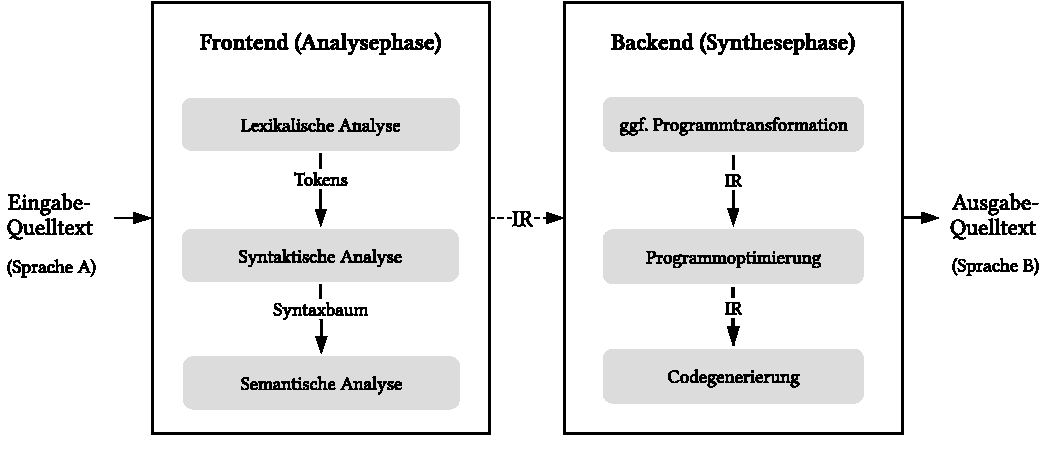
\includegraphics[width=\textwidth]{src/2_Grundlagen/fig/transpiler-architecture.pdf}
  \caption{Architektur eines typischen Transpilers nach~\autocite{EVGENIY:2016} und~\autocite[8]{TORCZON:2007}.}
	\label{fig:transpiler-architecture}
\end{figure}

Zunächst wird der Quelltext innerhalb der Analysephase durch den Lexer oder Tokenizer Zeichen für Zeichen eingelesen, um diesen in lexikalisch bedeutungsvolle Zeichenketten, sogenannte \emph{Lexeme} zu zerlegen~\autocite[43]{AHO:COMPILERS}. Daraufhin werden \emph{Tokens} gebildet, indem jedes dieser Wörter einer syntaktischen Klasse zugeordnet wird. Diese geben die Bedeutung eines Tokens an (zum Beispiel \code{3}~$\mapsto$~\code{INT(3)} oder \code{!=}~$\mapsto$~\code{NEQ})~\autocite[26]{TORCZON:2007}. Die Tokens entsprechen dabei den Terminalsymbolen der formalen Grammatik der Programmiersprache~\autocite[43]{AHO:COMPILERS}.

Im zweiten Schritt, der syntaktischen Analyse oder dem \emph{Parsen}, wird anschließend überprüft, ob die Tokenfolge eine Ableitung der kontextfreien Grammatik der Quellsprache darstellen, indem versucht wird einen entsprechenden \emph{konkreten} Syntaxbaum aufzubauen~\autocite{SCHOEPP:COMPILER}. Ein Syntax- oder Ableitungsbaum ist ein Graph, der die syntaktische Struktur eines Programms gemäß der zugehörigen Grammatik hierarchisch modelliert. Abbildung~\ref{fig:ast} zeigt exemplarisch den \emph{abstrakten} Syntaxbaum (AST) einer simplen JavaScript-Funktion. Ein abstrakter Syntaxbaum ist eine kompaktere Form des konkreten Baums und zeigt lediglich \enquote{wesentliche Teile}~\autocite[21]{WALDMANN:PPS} davon. Falls der Ableitungsbaum nicht erstellt werden kann, so liegt ein Syntaxfehler im Quelltext vor.

Danach prüft der Transpiler, ob ein gültiges Programm der Eingabesprache vorliegt, indem die statische Semantik analysiert wird~\autocite[8]{AHO:COMPILERS}. Hierunter fällt beispielsweise, dass Variablen in vielen Programmiersprachen vor deren Benutzung zunächst deklariert werden müssen. Um ein solches kontextuelles Programmverhalten zu untersuchen, können Attributgrammatiken verwendet werden~\autocite[161]{TORCZON:2007}. Während dieser Phase wird darüber hinaus die statische Typkorrektheit überprüft~\autocite{SCHOEPP:COMPILER}. Es ist hervorzuheben, dass nicht alle Transcompiler eine semantische Analyse durchführen.
Zuletzt wird durch das Frontend ein \emph{Zwischencode}\footnote{engl. \textit{intermediate representation} (IR).} des Programms erzeugt, der an das Backend übergeben wird. Ein Zwischencode ist im Allgemeinen eine von der Quellsprache und Zielarchitektur unabhängige Datenstruktur innerhalb von Compilern~\autocite[6]{TORCZON:2007}. Wie der nachfolgende Abschnitt zeigen wird, verwenden viele Transpiler im JavaScript-Umfeld den abstrakten Syntaxbaum als Zwischencode.

\begin{figure}[tb]
  {
    \begin{minted}{text}
function square(x) {
  return x ** 2;
}
    \end{minted}
    \vspace{-1.5cm}
    \begin{center}
      \ttfamily
      \begin{forest}
        [FunctionDeclaration
          [Identifier, edge label={node[edge]{id}}
            [square, edge label={node[edge]{name}}]
          ]
          [Identifier{[]}, edge label={node[edge]{params}}
            [x, edge label={node[edge]{name}}]
          ]
          [BlockStatement, for tree = {s sep=1.3cm}, edge label={node[edge]{body}}
            [ReturnStatement, edge label={node[edge]{body}}
              [BinaryExpression, edge label={node[edge]{argument}}
                [Identifier, edge label={node[edge]{left}}
                  [x, tier=last, edge label={node[edge]{name}}]
                ]
                [**, tier=last, edge label={node[edge]{operator}}]
                [Literal, edge label={node[edge]{right}}
                  [2, tier=last, edge label={node[edge]{value}}]
                ]
              ]
            ]
          ]
        ]
      \end{forest}
    \end{center}
  }
  \caption{Abstrakter Syntaxbaum der obigen JavaScript-Funktion gemäß der Spezifikation \textit{ESTree}~\autocite{ESTREE_SPEC}.}
  \label{fig:ast}
\end{figure}

Der erste Schritt der Synthesephase besteht darin, das Programm sprachunabhängig zu optimieren, das heißt die Laufzeit oder den Speicherplatzbedarf auf Grundlage von Programmanalyse zu reduzieren~\autocite[405]{TORCZON:2007}. Hierbei können eine Vielzahl unterschiedlicher Transformationen angewandt werden. Möglich ist zum Beispiel die Entfernung nicht erreichbarer Programmstücke (\textit{dead code elimination}) oder die Inline-Ersetzung von Konstanten und Schleifen~\autocites{TORCZON:2007}{SCHOEPP:COMPILER}. Auch hier gilt es zu betonen, dass nicht alle Transcompiler eine derartige Optimierungsphase besitzen. Schließlich kann im letzten Schritt der endgültige Quelltext in der Zielsprache auf Basis des gegebenenfalls optimierten Zwischencodes erzeugt werden~\autocite[505]{AHO:COMPILERS}.

\subsection{Evaluation bestehender Transpiler für JavaScript}
\label{subsec:js-transpilers}

\subsubsection{Anforderungen}

Im Umfeld von JavaScript sind im Lauf der Jahre eine Vielzahl von Parsern, Codegeneratoren und Transcompiler entstanden, welche die Entwicklung weiterer Werkzeuge wie die des angestrebten Flow-Transpilers stark vereinfachen können. Im Folgenden sollen die relevantesten, aktuellen Ansätze bezüglich verschiedener Aspekte gegenüber gestellt werden, sodass daraufhin die Entscheidung getroffen werden kann, welches der Werkzeuge als Grundlage für die Umsetzung heran gezogen wird. Hierbei wird lediglich frei verfügbare, quelloffene Software betrachtet.

Die Auswahl hängt entscheidend von der Erfüllung mehrerer technischer Anforderungen ab:
Der Parser muss aktuelle JavaScript-Syntax gemäß der ECMAScript-Spezifikation 2019~\autocite{ECMASCRIPT:2019} (ES2019) vollständig unterstützen.
Weiterhin muss die Verarbeitung von \emph{vorläufiger} Syntax möglich sein. Unter vorläufiger Syntax werden in dieser Arbeit vorgeschlagene Erweiterungen von JavaScript verstanden, die noch nicht endgültiger Bestandteil der Spezifikation sind, sondern sich noch im Standardisierungsprozess befinden\footnote{Die ECMAScript-Spezifikation wird stetig durch das \textit{Technical Committee 39} (TC39)~\autocite{TC39_COMMITTEE} weiterentwickelt. Vorgeschlagene Spracherweiterungen (\textit{ECMAScript proposals}) durchlaufen hierbei einen mehrstufigen Standardisierungsprozess, der schließlich in die Aufnahme in die Spezifikation münden kann~\autocite{TC39_PROCESS}.}. Die Anforderung derartige Syntax einlesen zu können ist ebenfalls eine Vorgabe, weil diese zum Teil bereits heute in der Praxis verwendet wird\footnote{Dies setzt die Benutzung eines Transpilers wie Babel voraus, der diese experimentelle Syntax vor der Auslieferung durch entsprechende Plugins in standardkonformes JavaScript transformiert.}.
Damit die Transpilierung von Flow nach TypeScript möglich ist, müssen einerseits jegliche Sprachkonstrukte von Flow verarbeitet werden können, andererseits muss das Format des abstrakten Syntaxbaums des Transpilers TypeScript vollständig unterstützen, sodass korrekter Ausgabequelltext erzeugt werden kann.
Aufgrund der gegebenen Rahmenbedingungen innerhalb des Unternehmens muss darüber hinaus sogenannte JSX-Syntax~\autocite{SOFTWARE:JSX} (\textit{JavaScript XML}) unterstützt werden, da die zu migrierenden Projekte diese Notation benutzen. Die Gründe für die Unterstützung von experimentellen Spracherweiterungen und von JSX werden in Abschnitt~\ref{subsec:requirement:syntax} ausführlich dargelegt.

\subsubsection{Vergleich}

% TODO: Auswertung Tabelle

% \bigbreak
\begingroup
\setlength{\tabcolsep}{6pt} % reset to default
\begin{table}[tb]
  \footnotesize
  \begin{tabu} to \textwidth {@{}lllccccccrrX@{}}
    \midrule
    \libertineSB{Werkzeug} & \libertineSB{Typ} & \libertineSB{Format} & \libertineSB{Erw.} & \libertineSB{ES10} & \libertineSB{ES10+} & \libertineSB{Flow} & \libertineSB{TS} & \libertineSB{JSX} & \libertineSB{Aktivität} & \libertineSB{Sterne} \\
    \midrule
    Acorn     & P  &  ESTree  & \pie{2} & \pie{2} & \pie{1} & \pie{0} & \pie{0} & \pie{2} &   5 &  5.250 & {\autocite{ACORN}} \\ % 2012
    Astring   & G  &  ESTree  & \pie{2} & \pie{2} & \pie{1} & \pie{0} & \pie{0} & \pie{0} &  61 &    500 & {\autocite{ASTRING}} \\ % 2015
    Babel     & PG &  Babel   & \pie{2} & \pie{2} & \pie{2} & \pie{2} & \pie{2} & \pie{2} & 225 & 34.650 & {\autocite{BABEL}} \\ % 2014
    Escodegen & G  &  ESTree  & \pie{0} & \pie{0} & \pie{0} & \pie{0} & \pie{0} & \pie{0} &   2 &  1.900 & {\autocite{ESCODEGEN}} \\ % 2012
    Esprima   & P  &  ESTree  & \pie{0} & \pie{1} & \pie{0} & \pie{0} & \pie{0} & \pie{1} &  12 &  5.450 & {\autocite{ESPRIMA}} \\ % 2011
    Recast    & PG &  diverse & \pie{2} & \pie{2} & \pie{2} & \pie{2} & \pie{2} & \pie{2} &  43 &  2.700 & {\autocite{RECAST}} \\ % 2012
    \midrule
  \end{tabu}
  \caption*{
    \footnotesize
    \begin{minipage}[t]{.4\linewidth}
      {
        \renewcommand{\arraystretch}{1.1}
        \begin{tabular}{@{}ll@{}}
          P & Parser\\
          G & Codegenerator\\
          \pie{0} & keine Unterstützung\\
          \pie{1} & unvollständige Unterstützung\\
          \pie{2} & vollständige Unterstützung\\
        \end{tabular}
      }
    \end{minipage}
    \begin{minipage}[t]{.55\linewidth}
      {
        \renewcommand{\arraystretch}{1.1}
        \begin{tabular}{@{}ll@{}}
          Erw. & Erweiterbarkeit\\
          ES10 & ECMAScript 2019\\
          ES10+ & vorgeschlagene JavaScript-Erweiterungen\\
          TS & TypeScript\\
          Sterne & Anzahl der Sterne auf GitHub\\
        \end{tabular}
      }
    \end{minipage}

    \medbreak
    \begin{justify}
      Aktivität: Entspricht der Summe der Zahl von \emph{Merge Requests}, neuer bzw. geschlossener Fehlerberichte, veröffentlichter Git-Commits auf dem Hauptzweig und der Anzahl beteiligter Autoren innerhalb eines Monats auf der Plattform GitHub~\autocite{GITHUB} (Stand Oktober 2019).
    \end{justify}
  }
  \caption{Vergleich verschiedener Werkzeuge zur Transpilierung von JavaScript"=Quelltexten.}
  \label{tab:transpilers}
\end{table}
\endgroup


% https://babeljs.io/blog/2016/12/07/the-state-of-babel#the-future-parser-unity
% https://medium.com/@sebmck/2015-in-review-51ac7035e272#.jdoo279bl

\subsubsection{Fazit}

Im Gegensatz zu den betrachteten Alternativen unterstützt lediglich Babel die Syntax von Flow, TypeScript und aktueller bzw. vorgeschlagener JavaScript-Sprachkonstrukte vollständig. Dieser Aspekt ist entscheidend, da nur so die geforderte universelle Übersetzung \emph{jeglicher} Flow-Syntax in äquivalentes TypeScript umgesetzt werden kann. Ein weiteres Argument für die Wahl von Babel ist einerseits die gute Erweiterbarkeit durch ein Plugin-System, andererseits die Ausgereiftheit und große Verbreitung des Projekts. Keine der anderen Optionen konnte die Anforderungen des Transpilers in vergleichbarem Maße erfüllen.

\subsection{Babel}
\label{sec:babel}

\subsubsection{Funktionsweise von Babel}

Zur Erleichterung des Verständnisses der Ausführung der Umsetzung des Flow-Transpilers in Kapitel \ref{chap:implementation} soll zunächst die grundsätzliche Funktionsweise von Babel umrissen werden. Die Ausführung von Babel gliedert sich in folgende drei Phasen~\autocite{BABEL:HANDBOOK}. Diese sind in weiten Teilen analog zu dem beschriebenen Aufbau eines typischen Transcompilers.

\begin{enumerate}
  \item {\libertineSB{Parsen des Eingabecodes}}\\*
    Zunächst wird der ursprüngliche Quelltext in zwei Schritten eingelesen, um den abstrakten Syntaxbaum des Programms zu erzeugen: Als Erstes wird der Code während der lexikalischen Analyse mittels des Lexers in Tokens zerlegt. Anschließend werden diese in der syntaktischen Analyse zu einer Datenstruktur umgeformt, die den zugehörigen abstrakten Syntaxbaum repräsentiert. Jedem Knoten des Baums wird dabei einen eindeutiger Tokentyp zugewiesen, der die syntaktische Bedeutung widerspiegelt.
    \bigbreak
  \item {\libertineSB{Transformation des Programms}}\\*
    Während der zweiten Phase wird daraufhin die eigentliche Programmtransformation durchgeführt: Dabei wird der abstrakte Syntaxbaum durch das \emph{Besucher}"=Entwurfsmuster\footnote{Das Besucher-Entwurfsmustern (engl. \textit{visitor pattern}) gehört zu den 23 Entwurfsmustern, die im Standardwerk \citetitle{GAMMA:1994} der \enquote{\textit{Gang of Four}} (E. Gamma, R. Helm, R. Johnson und J. Vlissides) beschrieben werden~\autocite[306\psqq]{GAMMA:1994}.} rekursiv traversiert und die Knoten des Baums sukzessive modifiziert, gelöscht bzw. neu erstellte Elemente eingefügt. Das Entwurfsmuster beschreibt, wie ein Algorithmus auf einer komplexen Objektdatenstruktur, unabhängig von der konkreten Implementierung der zugrunde liegenden Klassen, ausgeführt werden kann~\autocite[634\psq]{FREEMAN:2004}. Im vorliegenden Fall ermöglicht die Anwendung die individuelle Adressierung einer bestimmten Untermenge der Knoten des Syntaxbaums, sodass dort die gewünschte Transformation des Programms durchgeführt werden kann.
    \bigbreak
  \item {\libertineSB{Generierung des Ausgabequelltexts}}\\*
    Schließlich kann der Ausgabecode generiert werden: Hierbei werden alle Knoten des abstrakten Syntaxbaums durch Anwendung einer Tiefensuche durchlaufen und eine Zeichenkette aufgebaut, die den endgültigen, modifizierten Quelltext darstellt.
\end{enumerate}

\subsubsection{Babel-Plugins}
\label{subsec:babel-plugins}

Da die entscheidende Phase der Transpilierung, die Programmtransformation, bei Babel durch Plugins erzielt wird, sollen diese genauer betrachtet werden. Plugins sind die elementaren Bausteine, die eine flexible Erweiterung von Babel ermöglichen. Selbst der Kern des Transcompilers ist aus einer Vielzahl von Standard-Plugins zusammen gesetzt, die in ihrer Gesamtheit die Funktionalität des Systems abbilden~\autocite{BABEL}. Dies verdeutlicht die tiefgreifende Modularität der Architektur von Babel. Jedes Plugin ist eine JavaScript"=Funktion, welche gemäß der vorgegebenen Schnittstelle ein Objekt mit verschiedenen Attributen zurückliefern muss. Mindestens anzugeben ist dabei lediglich die Abbildung der gewünschten Knotentypen des abstrakten Syntaxbaums auf Besucherfunktionen~\autocite{BABEL:HANDBOOK}. Deren Implementierung setzt die angestrebte Quelltext"=Transformation um. Es ist in der Praxis gängig mehrere Plugins einzusetzen, sodass ein Knoten während der Verarbeitung durch Babel mehrere, unabhängige Transformationen durchlaufen kann. Hierdurch kann die erwünschte Transpilierung von JavaScript-Quelltexten flexibel durch Kombination vieler, kleiner Bausteine realisiert werden. Auch möglich ist die Angabe einer hierarchischen Abhängigkeitsstruktur, sodass dass die Verwendung eines Plugins zur impliziten Aktivierung weiterer Plugins führt.

Der konkrete Aufbau von Babel-Plugins soll durch ein Minimalbeispiel gezeigt werden. Quelltext~\ref{code:babel-plugin-definition} zeigt den Code eines simplen aber vollständigen Plugins, welches lediglich den Namen aller Bezeichner (\code{Identifier}) eines JavaScript-Programms in Großbuchstaben setzt. Hierfür wird eine gleichnamige Besucherfunktion für den Knotentyp \code{Identifier} definiert. Diese erhält den \emph{Pfad} der so adressierten Identifier-Knoten als Argument und kann diesen wie gewünscht transformieren. Der Pfad eines AST-Knotens ist ein Objekt, das die Beziehung des Knotens zu seinen Elternelementen modelliert und diesen um Metainformationen anreichert~\autocite{BABEL:HANDBOOK}. Es enthält eine Vielzahl von Methoden mittels derer der Pfad und der Syntaxbaum manipuliert werden kann.
Alle Knotentypen des abstrakten Syntaxbaums werden einerseits in der Spezifikation des Parsers von Babel~\autocite{BABEL:PARSER_SPEC,BABEL:PARSER}, andererseits in der Dokumentation der Bibliothek \code{@babel/types}~\autocite{BABEL:TYPES} beschrieben. Der Aufbau des von Babel eingesetzten abstrakten Syntaxbaums basiert auf dem Standard \textit{ESTree Spec}~\autocite{ESTREE_SPEC}. Dieser wird von Mitgliedern verschiedener Projekte im Umfeld der statischen Analyse von JavaScript kontinuierlich weiterentwickelt~\autocite{BABEL:PARSER,ESTREE_SPEC}. Grund für die Abspaltung Babels von der ESTree-Spezifikation seit Version 6 ist, dass das Projekt auch \emph{vorläufige} JavaScript-Erweiterungen unterstützen möchte~\autocite{BABEL:STATE_OF_BABEL}.

\bigbreak
\begin{listing}[htb]
\begin{textcode}
// var foo => var FOO
module.exports = function() {
  return {
    visitor: {
      Identifier(path) {
        path.node.name = path.node.name.toUpperCase();
      }
    }
  };
};
\end{textcode}
\listingvspace
\caption[Minimalbeispiel eines Babel-Plugins]{Minimalbeispiel eines Babel-Plugins: Die Namen aller Bezeichner (\code{Identifier}) werden in Großbuchstaben umgewandelt.}
  \label{code:babel-plugin-definition}
\end{listing}

Im weitere Verlauf wird das Hauptaugenmerk der Untersuchung auf die zweite Phase der Transpilierung gelegt, da hier die vorliegende Problemstellung, die Transformation der Flow-Typannotationen nach TypeScript, umgesetzt wird. Das Parsen des Eingabquelltexts und das Generieren der Ausgabe kann durch Verwendung der gegebenen Bibliotheksfunktionen von Babel simpel realisiert werden und bedarf keiner tiefgründigen Betrachtung.
